% Template for PLoS
% Version 3.5 March 2018
%
% % % % % % % % % % % % % % % % % % % % % %
%
% -- IMPORTANT NOTE
%
% This template contains comments intended
% to minimize problems and delays during our production
% process. Please follow the template instructions
% whenever possible.
%
% % % % % % % % % % % % % % % % % % % % % % %
%
% Once your paper is accepted for publication,
% PLEASE REMOVE ALL TRACKED CHANGES in this file
% and leave only the final text of your manuscript.
% PLOS recommends the use of latexdiff to track changes during review, as this will help to maintain a clean tex file.
% Visit https://www.ctan.org/pkg/latexdiff?lang=en for info or contact us at latex@plos.org.
%
%
% There are no restrictions on package use within the LaTeX files except that
% no packages listed in the template may be deleted.
%
% Please do not include colors or graphics in the text.
%
% The manuscript LaTeX source should be contained within a single file (do not use \input, \externaldocument, or similar commands).
%
% % % % % % % % % % % % % % % % % % % % % % %
%
% -- FIGURES AND TABLES
%
% Please include tables/figure captions directly after the paragraph where they are first cited in the text.
%
% DO NOT INCLUDE GRAPHICS IN YOUR MANUSCRIPT
% - Figures should be uploaded separately from your manuscript file.
% - Figures generated using LaTeX should be extracted and removed from the PDF before submission.
% - Figures containing multiple panels/subfigures must be combined into one image file before submission.
% For figure citations, please use "Fig" instead of "Figure".
% See http://journals.plos.org/plosone/s/figures for PLOS figure guidelines.
%
% Tables should be cell-based and may not contain:
% - spacing/line breaks within cells to alter layout or alignment
% - do not nest tabular environments (no tabular environments within tabular environments)
% - no graphics or colored text (cell background color/shading OK)
% See http://journals.plos.org/plosone/s/tables for table guidelines.
%
% For tables that exceed the width of the text column, use the adjustwidth environment as illustrated in the example table in text below.
%
% % % % % % % % % % % % % % % % % % % % % % % %
%
% -- EQUATIONS, MATH SYMBOLS, SUBSCRIPTS, AND SUPERSCRIPTS
%
% IMPORTANT
% Below are a few tips to help format your equations and other special characters according to our specifications. For more tips to help reduce the possibility of formatting errors during conversion, please see our LaTeX guidelines at http://journals.plos.org/plosone/s/latex
%
% For inline equations, please be sure to include all portions of an equation in the math environment.  For example, x$^2$ is incorrect; this should be formatted as $x^2$ (or $\mathrm{x}^2$ if the romanized font is desired).
%
% Do not include text that is not math in the math environment. For example, CO2 should be written as CO\textsubscript{2} instead of CO$_2$.
%
% Please add line breaks to long display equations when possible in order to fit size of the column.
%
% For inline equations, please do not include punctuation (commas, etc) within the math environment unless this is part of the equation.
%
% When adding superscript or subscripts outside of brackets/braces, please group using {}.  For example, change "[U(D,E,\gamma)]^2" to "{[U(D,E,\gamma)]}^2".
%
% Do not use \cal for caligraphic font.  Instead, use \mathcal{}
%
% % % % % % % % % % % % % % % % % % % % % % % %
%
% Please contact latex@plos.org with any questions.
%
% % % % % % % % % % % % % % % % % % % % % % % %

\documentclass[10pt,letterpaper]{article}
\usepackage[top=0.85in,left=2.75in,footskip=0.75in]{geometry}

% amsmath and amssymb packages, useful for mathematical formulas and symbols
\usepackage{amsmath,amssymb}

% Use adjustwidth environment to exceed column width (see example table in text)
\usepackage{changepage}

% Use Unicode characters when possible
\usepackage[utf8x]{inputenc}

% textcomp package and marvosym package for additional characters
\usepackage{textcomp,marvosym}

% cite package, to clean up citations in the main text. Do not remove.
\usepackage{cite}

% Use nameref to cite supporting information files (see Supporting Information section for more info)
\usepackage{nameref,hyperref}

% line numbers
\usepackage[right]{lineno}

% ligatures disabled
\usepackage{microtype}
\DisableLigatures[f]{encoding = *, family = * }

% color can be used to apply background shading to table cells only
\usepackage[table]{xcolor}

% array package and thick rules for tables
\usepackage{array}

% create "+" rule type for thick vertical lines
\newcolumntype{+}{!{\vrule width 2pt}}

% create \thickcline for thick horizontal lines of variable length
\newlength\savedwidth
\newcommand\thickcline[1]{%
  \noalign{\global\savedwidth\arrayrulewidth\global\arrayrulewidth 2pt}%
  \cline{#1}%
  \noalign{\vskip\arrayrulewidth}%
  \noalign{\global\arrayrulewidth\savedwidth}%
}

% \thickhline command for thick horizontal lines that span the table
\newcommand\thickhline{\noalign{\global\savedwidth\arrayrulewidth\global\arrayrulewidth 2pt}%
\hline
\noalign{\global\arrayrulewidth\savedwidth}}


% Remove comment for double spacing
%\usepackage{setspace}
%\doublespacing

% Text layout
\raggedright
\setlength{\parindent}{0.5cm}
\textwidth 5.25in
\textheight 8.75in

% Bold the 'Figure #' in the caption and separate it from the title/caption with a period
% Captions will be left justified
\usepackage[aboveskip=1pt,labelfont=bf,labelsep=period,justification=raggedright,singlelinecheck=off]{caption}
\renewcommand{\figurename}{Fig}

% Use the PLoS provided BiBTeX style
\bibliographystyle{plos2015}

% Remove brackets from numbering in List of References
\makeatletter
\renewcommand{\@biblabel}[1]{\quad#1.}
\makeatother



% Header and Footer with logo
\usepackage{lastpage,fancyhdr,graphicx}
\usepackage{epstopdf}
%\pagestyle{myheadings}
\pagestyle{fancy}
\fancyhf{}
%\setlength{\headheight}{27.023pt}
%\lhead{\includegraphics[width=2.0in]{PLOS-submission.eps}}
\rfoot{\thepage/\pageref{LastPage}}
\renewcommand{\headrulewidth}{0pt}
\renewcommand{\footrule}{\hrule height 2pt \vspace{2mm}}
\fancyheadoffset[L]{2.25in}
\fancyfootoffset[L]{2.25in}
\lfoot{\today}

%% Include all macros below

\newcommand{\lorem}{{\bf LOREM}}
\newcommand{\ipsum}{{\bf IPSUM}}

%% END MACROS SECTION


\begin{document}
\vspace*{0.2in}

% Title must be 250 characters or less.
\begin{flushleft}
{\Large
\textbf\newline{Title of submission to PLOS journals} % Please use "sentence case" for title and headings (capitalize only the first word in a title (or heading), the first word in a subtitle (or subheading), and any proper nouns).
}
\newline
% Insert author names, affiliations and corresponding author email (do not include titles, positions, or degrees).
\\
Vincent Ragusa\textsuperscript{1*},
Matthew Andres Moreno\textsuperscript{1},
Rachel Greenberg\textsuperscript{2}
\\
\bigskip
\textbf{1} BEACON Center, Michigan State University, East Lansing, MI, USA
\\
\textbf{2} Department of Microbiology \& Molecular Genetics, Michigan State University, East Lansing, MI, USA
\\
\bigskip

% % Insert additional author notes using the symbols described below. Insert symbol callouts after author names as necessary.
% %
% % Remove or comment out the author notes below if they aren't used.
% %
% % Primary Equal Contribution Note
% \Yinyang These authors contributed equally to this work.
%
% % Additional Equal Contribution Note
% % Also use this double-dagger symbol for special authorship notes, such as senior authorship.
% \ddag These authors also contributed equally to this work.

% Current address notes
% \textcurrency Current Address: Dept/Program/Center, Institution Name, City, State, Country % change symbol to "\textcurrency a" if more than one current address note
% \textcurrency b Insert second current address
% \textcurrency c Insert third current address

% Deceased author note
%\dag Deceased

% Use the asterisk to denote corresponding authorship and provide email address in note below.
* ragusavi@msu.edu

\end{flushleft}
% Please keep the abstract below 300 words
\begin{abstract}
% Abstract length should not exceed 250 words
%One or two sentences providing a basic introduction to the field, comprehensible to a scientist in any discipline
Stigmergy is an indirect mechanism of coordination where an action alters the environment and the changed environment, in turn, alters the likelihood of future actions.
Pheromone, marker-based, stigmergy is the most common form of stigmergy used in social insect groups.
%Two to three sentences of more detailed background, comprehensible to scientists in related disciplines
The ant species \textit{Monomorium pharaonis} is known to produce both an attractive and repellent pheromone marker allowing for both positive and negative feedback.
Additionally,\textit{Monomorium pharaonis} produces pheromones that decay after several minutes, whereas \textit{Atta columbica} produce pheromones that persist for several years.
It has been hypothesized that the vast range of decay rates may be linked to the stability of the species’ food source.
%One sentence clearly stating the general problem being addressed by this particular study
However, the precise environmental conditions necessary to drive evolution toward the use of stigmergy as a form of navigational coordination is unknown.
%One sentence summarizing the main result (with the words “here we show” or their equivalent).
Here we use digital agent-based evolution to show that a moderate pheromone decay rate corresponds with an increase in likelihood that an agent evolves a stigmergic foraging strategy.
%Two or three sentences explaining what the main result reveals in direct comparison to what was thought to be the case previously, or how the main result adds to previous knowledge.
X
X
X
%One or two sentences to put the results into a more general context
Y
Y
%Two or three sentences to provide a broader perspective, readily comprehensible to a scientist in any discipline
Z
Z
Z
\end{abstract}


\section{Introduction}

Power law distributions in Nature usually signal the absence of a
scale in the region where the scaling is observed, and sometimes point
to critical dynamics. In Self-Organized-Criticality (SOC)
\citep{BTW87,BTW88}, for example, power law distributions reveal the
dynamics of an unstable critical point, brought about by slow driving
and a feed-back mechanism between order parameter and critical
parameter.  The critical dynamics is usually described within the
language of second-order phase transitions in condensed matter systems
\citep{SJD}, but it can be shown that SOC-type behavior also occurs
within a dual description in terms of the Landau-Ginzburg equation as
{\em first-order} transitions \citep{GS}.  Indeed, it was shown that a
power law distribution of {\em epoch-lengths}, that is, the time a
particular species dominates the dynamics of an adapting population,
is explained by a self-organized critical scenario \citep{CA2} that
carries the hallmark of first-order phase transitions. Here, we
measure the distribution of abundances of {\em species} and genotypes
in an artificial chemistry, \citep[the Avida Artificial Life
system][]{AB1,OBA} and show that the distribution is scale-free under
a broad class of circumstances, confirming the results reported in
\citep{CA2}.  In the next section, we discuss the first-order dynamics
in more detail and examine ``avalanches of invention'' from the point
of view of a thermodynamics of information. In Section III, we measure
the critical exponent of the power law of genotype abundances in the
limit of infinitesimal driving, i.e., infinitesimal mutation rate, and
discuss the role of the fitness landscape in shaping the
distribution. In Section IV, we repeat the analysis for a higher
taxonomic level (that of species) and discuss its relation to the
geometric distributions found by \citet{BUR90,BUR93}.
Conclusions about the evolutionary process drawn from the data
obtained in this paper are presented in Section V.


\section{Methods}

\subsection{MABE}\label{mabe}

In this work, we use the Modular Agent-Based Evolver\cite{bohm_mabe_2017} (MABE) framework to build and run our experiments. MABE allows for the quick construction of agent-based evolution simulations by allowing the scientist to reuse aspects of the system that have already been built by other members of the MABE community. In our work, we use the modules for Markov Brains, Circular Haploid Genomes, simple mutation-only reproduction via roulette selection, and population data archiving. Our programming effort is therefore minimized to simply creating the world module, the module that defines the environment the agent will be evaluated in.

\subsection*{Markov Brains}

We used Markov brains in this work as the evolved controller of our agents. The Markov brains used here consist of four major components: The input vector, output vector, hidden vector, and logic gates. The first three components are simply vectors of values, typically bits, that the gate components can read from and write to. The size of the input, output, and hidden vectors must be decided before the brain is built. The sizes of the input and output vectors are determined by the world module (Section \ref{world}). The size of the hidden vector is independent and is a tunable parameter.

The gates of the agent's Markov brain are, typically, binary logic gates whose input nodes, output nodes, and internal logic are all determined by interpreting the agent's genome. This genome-to-gates interpretation is all handled within MABE's Markov brain module. Gates read from and write to any input, output, or hidden node specified by the genome. Gates can have between 0 and 4 input connections and between 0 and 4 output connections. The smallest functional gate is, therefore, a one-in-one-out gate whose logic can take on 4 unique logic tables. The largest gate possible is a four-in-four-out gate with 256 potential logic tables.

In this work, we also use trit gates, which work the same as the binary gates described above, with the added benefit that trits can take on a third value, $-1$, which can provide useful down-regulation within the brain. Additionally, the one-in-one-out trit gate capable of 9 logic tables while the four-in-four-out trit gate has 6561.

\subsection {Stigmergy World} \label{world}

The world module in MABE is responsible for defining three key aspects of the simulation: The environment, how the agent senses the environment, and how the agent can change the environment.

\subsection*{Map Generation}

In this work, the environment is an $n\times m$ grid surrounded by a wall and filled with smaller wall segments that create obstructions for the agent to navigate around. In addition, the environment contains one home location, where the agent will begin each simulation, and a food location. The environment is constructed by first generating a maze and then removing walls until the desired density of obstacles is reached (Figure \ref{fig:world_explanatory}). This method was chosen to ensure that home and food locations are always reachable by some path through the obstacles.

\begin{figure}
\begin{center}
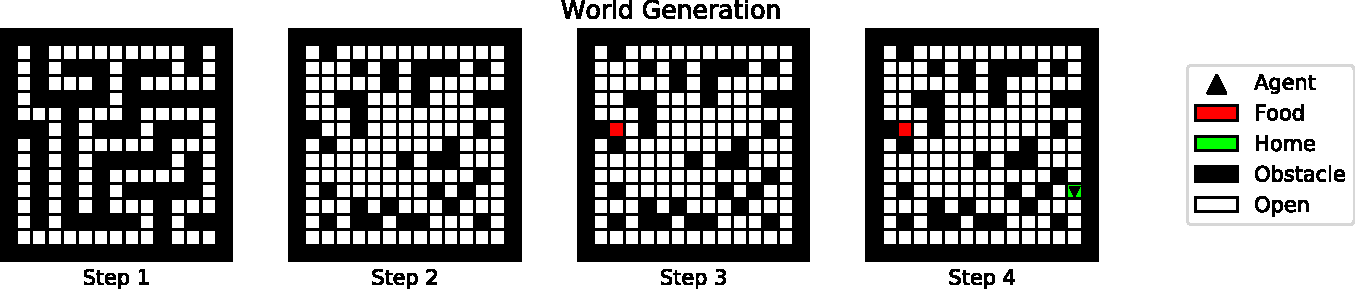
\includegraphics[width=\textwidth]{img/world_explanatory}
\caption{
Caption TODO
}
\label{fig:world_explanatory}
\end{center}
\end{figure}


The maze layout, walls removed, home location, and initial food location are all generated/chosen randomly during environment construction. A new environment is created before every agent evaluation. Furthermore, the location of food may change during an agent's lifetime according to the rules for food use (see Fitness Function). When the food must move, it is randomly relocated.

\subsection*{Agent Inputs}

The agent is equipped with a total of $43+k$ bits of sensor data (Figure \ref{fig:sense_explanatory}). The agent has a vision cone that covers 8 cells and the capability of distinguishing 4 environmental states at each location (32 bits), a $3\times 3$ stigmergy proximity sensor centered on the agent's location (9 bits), an internal compass that provides a two-bit representation of the four cardinal directions, and a stigmergy read sensor that senses the $k$ bit stigmergy signal. In this work we have set $k$ to be $1$, disallowing the agent access to multiple, distinguishable, stigmergy signals. The agent receives input from each of its sensors at every world update.

\begin{figure}
\begin{center}
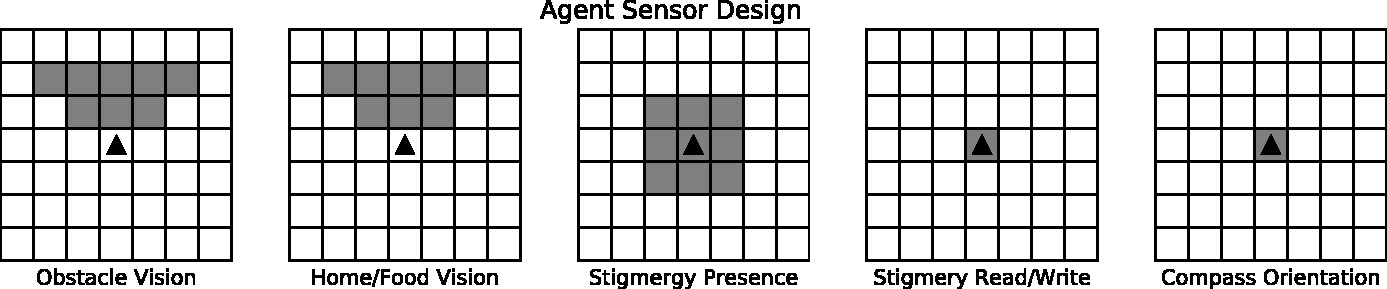
\includegraphics[width=\textwidth]{img/sense_explanatory}
\caption{
The agent's sensors' ranges of influence are indicated by the shaded locations. Left to Right: Agent vision cone wall, food, and home components; Agent pheromone proximity sensor; Agent pheromone secretion and discrimination location; and agent compass.
}
\label{fig:sense_explanatory}
\end{center}
\end{figure}


\subsection*{Agent Outputs}

The agent has a total of $2+k$ output bits. The agent moves throughout the environment via tank controls (Figure \ref{fig:movement_explanatory}) (2 bits). The agent can make no movement by outputting $00$ to the movement bits. The agent also writes $k$ bits to the current location in the form of a stigmergy signal. Writing all zeros is the same as writing no signal. The agent will always output signal on every world update, however, it can choose to do nothing by writing zeros to the move bits, stigmergy bits, or all output bits. Recall that we have set $k$ to be $1$ in this work, so the agent can only write a single kind of signal or write no signal.

\begin{figure}[!htbp]
\begin{center}
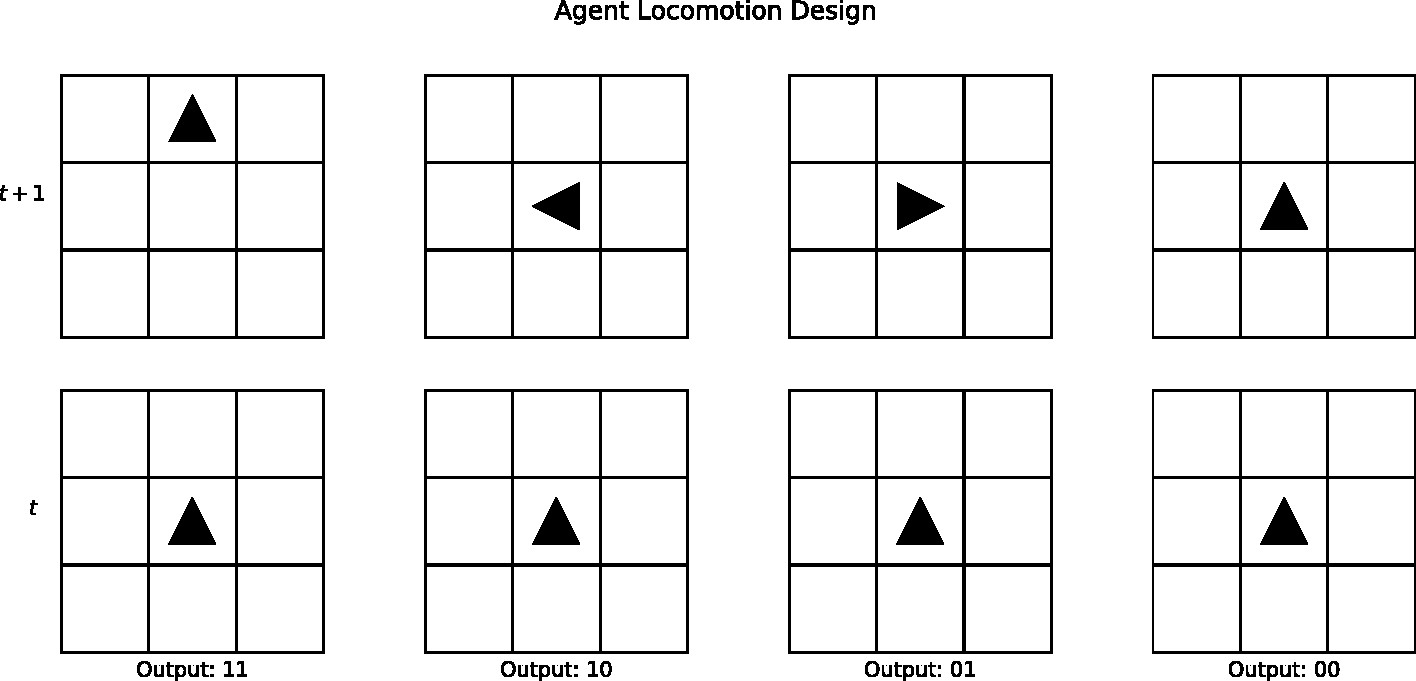
\includegraphics[width=\textwidth]{img/movement_explanatory}
\caption{
Caption TODO
}
\label{fig:movement_explanatory}
\end{center}
\end{figure}


\subsection*{Agent Fitness Function}

During its lifetime (1000 world updates), each agent is tasked with foraging for food, indicated by the food marker on the grid, and returning to the home location with some of it. Each time the agent picks up a piece of food, by stepping on the food location, it adds $+1$ to its fitness. If the agent successfully returns home with the food in hand, the agent adds $+10$ to its fitness. The food location will provide food to the agent a random number of times, between 5 and 10, and then change location on the map. The agent who can quickly locate food, and efficiently make trips between the food and its home, will achieve the highest fitness. Furthermore, each time the agent takes a step forward or places a stigmergic pheromone, the agent receives $+0.001$ fitness. Over the course of the agent's lifetime, these minor fitness payouts can sum to no greater than $2$ points. These small fitness payouts are there to encourage agents to use their outputs and begin walking or secreting pheromone early in the evolutionary run but are kept small enough that once an agent is capable of scoring points from foraging these minor payouts will be negligible to selection.

\subsection {Experimental Design}

Our goal with this work is to investigate how pheromone evaporation rate affects the fitness of evolved foraging strategies and the degree to which these evolved strategies depend on stigmergy. We hypothesize that evaporation rates that are too extreme, either too slow or too fast, will have low fitness and reduce selective pressure on the use of stigmergy.

To test this hypothesis, we first explore the parameter space of our world to determine where agents evolve the fittest strategies without stigmergy. We then use these parameter values to conduct the final experiment with stigmergy. This is done to help mitigate the possibility that stigmergic strategies evolve primarily due to a fundamental limitation on the agent's ability to solve the problem without it.

All agents are evaluated five times in a generation and their scores from these five evaluations are averaged and reported as the agent's fitness for that generation. This is done to help ensure that agents who are placed in an environment that is exceedingly complimentary to their current strategy do not benefit from this lucky event. Rather, agents must have a strategy that is fit, on average, in 5 different environments, reducing the probability of fixation of lucky but generally unfit agents.

\subsection*{Obstacle Density}

As discussed in section \ref{world}, the environment is generated by first building a maze and then randomly removing walls. The percentage of walls that are removed can be varied between 0.00, or a complete maze, and 1.00, an empty $n-1 \times m-1$ grid surrounded by walls. We evolve our agents in environments characterized by 0.00, 0.20, 0.40, 0.60, 0.80, and 1.00 percent wall removal.

\subsection*{Agent Memory}

As discussed in section \ref{mabe}, we used the Markov Brain MABE module to control our agents’ behavior. Markov brains can have any number of hidden nodes which provide the brain with the capability of internal memory. However, too few hidden nodes might make the agent incapable of evolving a fit strategy to a complex problem like stigmergy world, yet too many can make the process of evolution far too slow to do meaningful science. Therefore, we evolve agents that have 0, 1, 2, 4, 8, 16, 32, 64, and 128 hidden nodes to determine where agents are most fit.

\subsection*{Stigmergic Chemical Evaporation Rate}

With the previous two tests completed, we conduct our main experiment to determine how pheromone evaporation affects evolved foraging strategies and to what degree these strategies depend on the use of these pheromones as stigmergic signals. The pheromone evaporation rate is given in units of world updates. We evolved agents with evaporation rates of 1000, 500, 100, 50, 10, 5, and 1. The evaporation rate of 1000 corresponds to permanent pheromone placement, and 1 corresponds to immediate evaporation.

\subsection*{Implementation}

The code used to perform and analyze our experiments, our figures, data from our experiments, tutorials describing how to repeat our experiments and analyses, and video demonstrations of evolved agent behaviors are available via the Open Science Framework at \url{https://osf.io/ydtvs/}.
Each 20,000 generation evolutionary replicate ran approximately four hours on a single-core compute node.
In total, experiments reported consumed roughly 16,000 compute hours.

With the previous two tests completed, we conduct our main experiment to determine how pheromone evaporation affects evolved foraging strategies and to what degree these strategies depend on the use of these pheromones as stigmergic signals. The pheromone evaporation rate is given in units of world updates. We evolved agents with evaporation rates of 1000, 500, 100, 50, 10, 5, and 1. The evaporation rate of 1000 corresponds to permanent pheromone placement, and 1 corresponds to immediate evaporation.


\section{Results}

\begin{figure}[!htbp]
\begin{center}
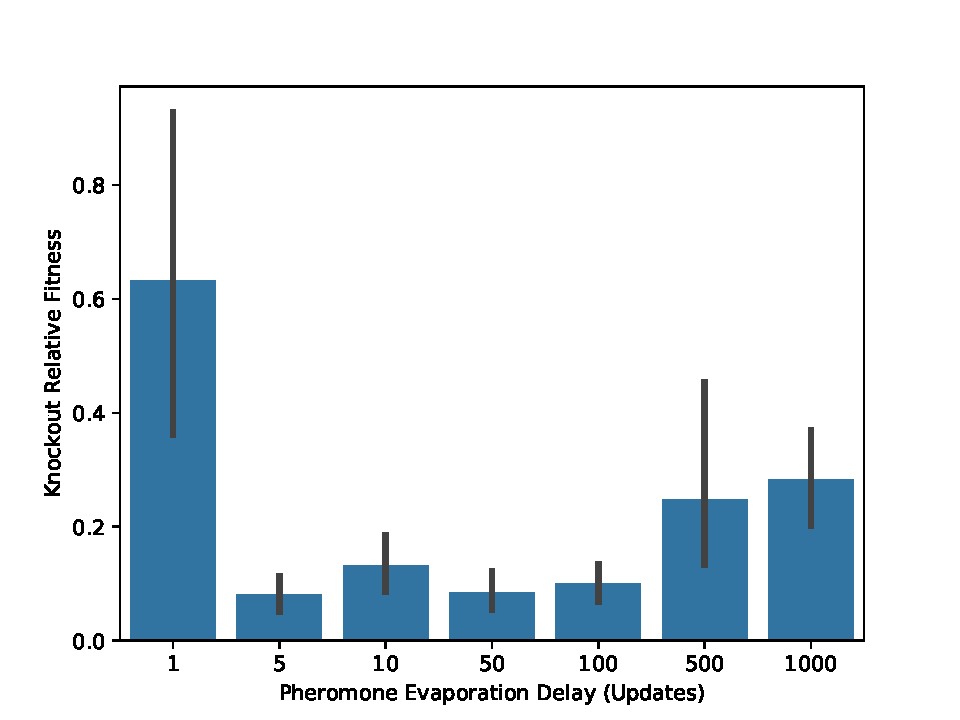
\includegraphics[width=\textwidth]{img/knockout_rel_fit_stig_delay.pdf}
\caption{
Caption TODO
}
\label{fig:knockout_rel_fit_stig_delay}
\end{center}
\end{figure}


\subsection{Obstacle Density}

\subsection{Agent Memory}

\subsection{Stigmergic Chemical Evaporation Rate}


\section{Discussion}


\section{Conclusion}

Our observation of maximal foraging performance at intermediate stigmergy evaporation rates qualitatively concurs with results from existing models with manually-designed navigation strategies \cite{panait2004ant}.
Interestingly, the evolutionary component of our model suggests that although evolved behavior cannot fully overcome the limitations of too-slow or too-fast stigmergy evaporation, evolved navigation strategies appear to compensate by relying less heavily on stigmergic cues.
This result shows that the extent to which stigmergic cues govern evolved foraging behavior can vary progressively.
This suggests, perhaps, that transitions to or from behavioral reliance on stigmergic cues need not be viewed as a on-or-off leap.

In future work, we will investigate the relationship between stigmergic volatility and food source permanence noted in \textit{Monomorium pharaonis} and \textit{Atta columbica} \cite{jeanson_pheromone_2003, howard_costs_2001, robinson_decay_2008}.
We expect to observe greater evolved foraging performance is achieved at low stigmergy volatility for permanent food placement and whether greater evolved foraging performance is observed at high stigmergy volatility for transient food placement.
These experiments will help confirm the functional implications of stigmergy volatility with respect to ask switching suggested by biological observation and shed light on the evolutionary roots of these differences in stigmergy volatility.


\section{Acknowledgements}

We would like to thank Chris Adami, Wolfgang Banzhaf, Arend Hintze, and Charles Ofria for their guidance and advice.

We would also like to thank Cliff Bohm for helping us use the MABE framework to conduct our research.

We performed this work in the Multidisciplinary Approaches to the Study of Evolution course sponsored by the NSF BEACON Center for the Study of Evolution in Action.

This work was supported in part by Michigan State University through computational resources provided by the Institute for Cyber-Enabled Research.


\nolinenumbers

\bibliography{bibl}

\end{document}
